%%%%%%%%%%%%%%%%%%%%%%%%
% Downloading the EMTG Git Repository
%%%%%%%%%%%%%%%%%%%%%%%%

\begin{enumerate}
	\item Navigate to \url{https://github.com/nasa/EMTG/}.
	\item Verify that the branch selected is master
		\begin{figure}[H]
			\centering
			
\includegraphics[width=0.5\linewidth]{../../../shared_latex_inputs/images/emtg_github_master_select.png}
			\caption{GitHub Master Branch Selection}
		\end{figure}
	\item Download the zip file by clicking the ‘Code’ button, select the ‘Download Zip’ option, and save to your desired location. Note that cloning the git repository is also an option, but this guide focuses on the simpler method of downloading a static copy of the repository using the `Download Zip' option. 
		\begin{figure}[H]
			\centering
			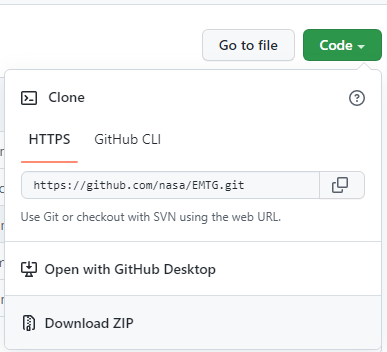
\includegraphics[width=0.5\linewidth]{../../../shared_latex_inputs/images/emtg_github_code_download.png}
			\caption{GitHub Download Prompt}
		\end{figure}
	\begin{enumerate}
		\item The user should save this directory to their local machine into a destination with no spaces in the file path and record its location for future use (e.g. C:\textbackslash SW\_Installs\textbackslash EMTG).
	\end{enumerate}
	\item Locate the folder that contains the ‘EMTG-Config-template.cmake’ file. \\ For the remainder of this document, this folder will be identified as \textbf{\textless EMTG\_root\_dir\textgreater}	
	\item Create the \textbf{\textless EMTG\_root\_dir\textgreater}\textbackslash HardwareModels\textbackslash \hspace{1pt} folder
	\item Copy the default.emtg\_launchvehicleopt and empty.ThrottleTable files from the \\ \textbf{\textless EMTG\_root\_dir\textgreater}\textbackslash testatron\textbackslash HardwareModels\textbackslash to the \\ \textbf{\textless EMTG\_root\_dir\textgreater}\textbackslash HardwareModels\textbackslash \hspace{1pt} folder
	\item Create the \textbf{\textless EMTG\_root\_dir\textgreater}\textbackslash Universe\textbackslash \hspace{1pt} folder
	\item Create the \textbf{\textless EMTG\_root\_dir\textgreater}\textbackslash Universe\textbackslash ephemeris\_files\textbackslash \hspace{1pt} folder
	\item Copy the *.emtg\_universe files from the  \textbf{\textless EMTG\_root\_dir\textgreater}\textbackslash testatron\textbackslash universe\textbackslash \hspace{1pt} folder to the \textbf{\textless EMTG\_root\_dir\textgreater}\textbackslash Universe\textbackslash \hspace{1pt} folder
	\item Copy the default.emtg\_universe.emtg\_universe file from the \textbf{\textless EMTG\_root\_dir\textgreater}\textbackslash PyEMTG\textbackslash \hspace{1pt} folder to the \textbf{\textless EMTG\_root\_dir\textgreater}\textbackslash Universe\textbackslash \hspace{1pt} folder and rename to Sun\_barycenters.emtg\_universe
\end{enumerate}